\section{Ablation}
\label{sec:ablation}

\subsection{What was varied}
\label{sec:ablation-setup}

The wrapper has three components that a validator can set: the step $\gamma$ of the level update, the band of the working level, and the ES that accompanies the recalibrated VaR (\cref{sec:method-decisions}). \Cref{tab:ablation} changes one at a time on HS-250, GARCH-t and FHS at both levels in the three stress windows, which makes 18 cells per row. The row for $\gamma = 0$ is the unwrapped model and the row for the default is the wrapper whose results fill \cref{sec:results}. The same forecaster context serves every row of a model-window pair, so the rows differ only by the component changed. The mean score change is taken over the cells with respect to the unwrapped row, and the worst score change is the largest single cell; $Z_2$ is the mean of the Acerbi--Szekely statistic over the cells.

\begin{table}[htbp]
\centering
\small
\caption{Ablation of the wrapper on HS-250, GARCH-t and FHS at two tail levels in the three stress windows (18 cells): each row changes one component of the full wrapper (the step, the clipping band of the working level, the ES paired with the recalibrated VaR) and keeps the others. $Z_2$ is the Acerbi--Szekely statistic, zero for a correct ES and negative for an understated one; clipped days count updates cut by the band.}
\label{tab:ablation}
\begin{adjustbox}{max width=\textwidth}
\begin{tabular}{lrrrrrrr}
\toprule
Variant & Cells passing & Independence failures & Mean $|$hit $-$ target$|$ (points) & Mean FZ0 change & Worst FZ0 change & Mean $Z_2$ & Clipped days \\
\midrule
\relax Unwrapped ($\gamma = 0$) & 6 / 18 & 1 & 3.08 & \relax +0.0\% & \relax +0.0\% & -2.28 & 0 \\
\relax Full wrapper ($\gamma = 0.005$) & 15 / 18 & 0 & 1.20 & \relax -47.1\% & \relax +3.4\% & -1.11 & 37 \\
\relax Step $\gamma = 0.001$ & 10 / 18 & 0 & 2.35 & \relax -15.4\% & \relax +0.8\% & -1.77 & 3 \\
\relax Step $\gamma = 0.0025$ & 15 / 18 & 0 & 1.61 & \relax -29.7\% & \relax +1.4\% & -1.33 & 15 \\
\relax Step $\gamma = 0.01$ & 15 / 18 & 0 & 1.02 & \relax -56.0\% & \relax +10.9\% & -1.02 & 64 \\
\relax Step $\gamma = 0.02$ & 14 / 18 & 0 & 1.24 & \relax -59.1\% & \relax +22.3\% & -1.21 & 94 \\
\relax Step $\gamma = 0.05$ & 10 / 18 & 0 & 1.91 & \relax -52.6\% & \relax +47.2\% & -1.74 & 171 \\
\relax Band $[10^{-5}, 0.5]$ & 15 / 18 & 0 & 1.19 & \relax -45.8\% & \relax +3.4\% & -1.09 & 30 \\
\relax Band $[\alpha/2, 2\alpha]$ & 12 / 18 & 0 & 1.96 & \relax -28.1\% & \relax +2.8\% & -1.59 & 115 \\
ES keeps the target ES/VaR ratio & 15 / 18 & 0 & 1.20 & \relax -50.1\% & \relax +3.6\% & -1.00 & 37 \\
ES left at the target level & 15 / 18 & 0 & 1.20 & \relax -45.4\% & \relax +3.0\% & -1.21 & 37 \\
\bottomrule
\end{tabular}
\end{adjustbox}
\end{table}


\subsection{The step is the component that matters}
\label{sec:ablation-step}

Without the update the three models pass \ablOffPass{} of \ablOffN{} cells; with the default step they pass \ablFullPass{}. A step five times smaller (0.001) gives \ablGammaAPass{}: the level moves too slowly to follow a regime that lasts a few hundred days, and the mean distance of the hit rate from its target stays at \ablGammaADev{} points against \ablFullDev{} for the default. Steps of 0.0025, 0.005 and 0.01 pass the same number of cells (\ablGammaBPass{}, \ablFullPass{} and \ablGammaCPass{}), and the hit rate approaches its target further as the step grows (\ablGammaBDev{}, \ablFullDev{} and \ablGammaCDev{} points). Beyond 0.01 the passes fall (\ablGammaDPass{} at 0.02 and \ablGammaEPass{} at 0.05), and the mean distance of the hit rate from its target rises again (\ablGammaDDev{} and \ablGammaEDev{} points), consistent with a level that fluctuates too much, and the score pays for it: the worst change of the mean score is \ablGammaBFzWorst\% at 0.0025, \ablFullFzWorst\% at the default, \ablGammaCFzWorst\% at 0.01, \ablGammaDFzWorst\% at 0.02 and \ablGammaEFzWorst\% at 0.05. The tolerance of 5\% is respected by the steps up to the default and broken by the larger ones, so the range between 0.0025 and the default is the one where the cells passed are at their maximum and the score cost is within the tolerance. The number of days on which the band acts rises with the step, from \ablGammaAClip{} days at 0.001 to \ablGammaEClip{} at 0.05 (\cref{fig:gamma-sweep}). The default of the engine, which was fixed before any stress window was run, is inside that range; the result is a property of the three-window test and of the three models, and a different set of windows could place the best step elsewhere. The cells passed in this ablation are counted with the engine's tests, which accept a count held near its target too easily (\cref{sec:results-dispersion}); up to a step of 0.01 a larger step holds the count tighter, and beyond it the band acts on more days and the count moves away from its target again (\ablGammaCDev{}, \ablGammaDDev{} and \ablGammaEDev{} points at 0.01, 0.02 and 0.05). The distance of the hit rate from its target, which does not enter the tests, is the figure to read for the ranking of the steps (smallest at 0.01, \ablGammaCDev{} points, then at the default, \ablFullDev{}).

\begin{figure}[htbp]
\centering
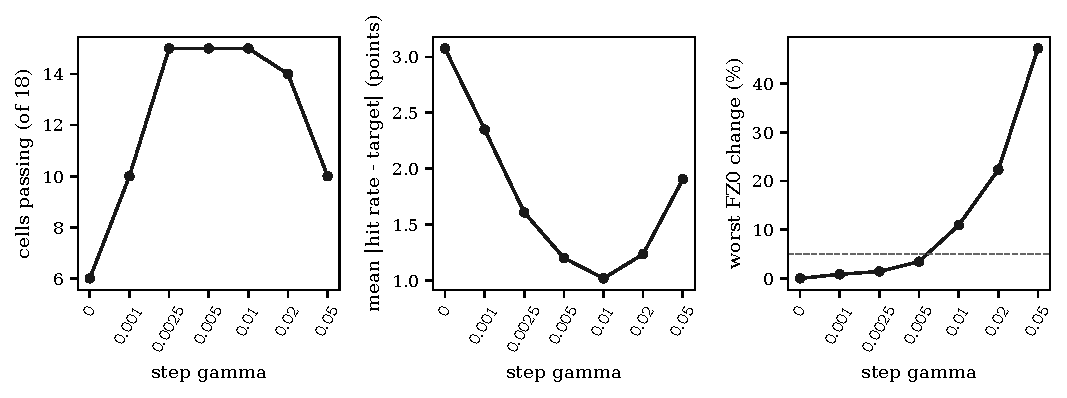
\includegraphics[width=\textwidth]{gamma-sweep}
\caption{Effect of the step $\gamma$ of the level update on HS-250, GARCH-t and FHS at two levels in the three stress windows (18 cells): cells passing the Kupiec and conditional coverage tests (left), mean distance of the hit rate from its target in percentage points (centre) and the worst relative change of the mean FZ0 score (right, the dashed line being the 5\% tolerance); the first point, 0, is the unwrapped model.}
\label{fig:gamma-sweep}
\end{figure}

\subsection{The band and the paired ES matter little at this scale}
\label{sec:ablation-band-es}

Widening the band to $[10^{-5}, 0.5]$ changes nothing in the count of cells passed (\ablBandWidePass{}) and leaves the worst score change at \ablBandWideFzWorst\%; the clipped days fall from \ablFullClip{} to \ablBandWideClip{}. Narrowing it to $[\alpha/2, 2\alpha]$ costs three cells (\ablBandNarrowPass{} passed) and raises the mean distance of the hit rate to \ablBandNarrowDev{} points, with \ablBandNarrowClip{} clipped days: a band that is too tight does not let the level reach the value at which the model is right, which is the content of \cref{prop:fixed-point}(c). The default band is therefore wide enough for these windows and need not be wider; no cell failed because of it, except in the scale sweep, where the band limits the repair (\cref{tab:scale-sweep}).

The two alternatives to the model's own tail mean as the ES do not change the coverage, as they should not (the VaR is the same), and change the ES calibration slightly: the mean $Z_2$ is \ablFullZtwo{} for the default, \ablEsRatioZtwo{} when the ES keeps the model's ratio to the VaR at the target level, and \ablEsTargetZtwo{} when it is left at the target level, with worst score changes of \ablEsRatioFzWorst\% and \ablEsTargetFzWorst\%. The differences are of the order of 0.1 in $Z_2$ and 0.6 percentage points in the score, and the experiment gives no interval for them; the decision to use the model's own ES at the working level rests on its coherence with the VaR (both come from one distribution) and not on a measured advantage.

\subsection{What each component contributes}
\label{sec:ablation-summary}

Reading the table as a decomposition, the update itself contributes the whole gain in cells passed: from \ablOffPass{} to \ablFullPass{} of \ablOffN{}, with no independence failure introduced (\ablFullInd{} failures against \ablOffInd{} unwrapped). The step sets how fast the gain is reached and how much score it costs, with an interior range of good values. The band bounds the repair and matters when it is too narrow. The paired ES is a matter of convention within the precision of these windows. None of the variants repairs the ES: the mean $Z_2$ stays between \ablEsRatioZtwo{} and \ablGammaAZtwo{} in all of them, against \ablOffZtwo{} for the unwrapped models.

Two limits of the decomposition follow from its design. The components were changed one at a time, so an interaction (a wider band with a larger step, say, which would let a fast level reach deeper before it is cut) was not measured. The counts of cells passed are counts over 18 cells that share the days of three windows, and a difference of one or two cells, such as the one between the steps 0.01 and 0.02, is within what a change of a few hits would move; the ordering of the steps is read from the pattern over the whole sweep of \cref{fig:gamma-sweep} and not from any single neighbouring pair.
